\documentclass[11pt,a4paper]{article}
% Közös preambulum a kézikönyvhöz és a programfelépítéshez
\usepackage[utf8]{inputenc}
\usepackage[T1]{fontenc}
\usepackage[magyar]{babel}
\usepackage{lmodern}
\usepackage{microtype}
\usepackage[a4paper,margin=2.3cm]{geometry}
\usepackage{graphicx}
\usepackage{booktabs,array,longtable,tabularx}
\usepackage{xcolor}
\usepackage{listings}
\usepackage{amsmath,amssymb}
\usepackage{textcomp}
\usepackage{csquotes}
\usepackage{enumitem}
\usepackage{caption}
\usepackage[most]{tcolorbox}
\usepackage{tikz}
\usetikzlibrary{arrows.meta,positioning,shapes.geometric,fit,calc,backgrounds}
\usepackage[hidelinks]{hyperref}

\graphicspath{{../img/}}
\newcommand{\rootdir}{../../..}
\setlist{itemsep=2pt,topsep=4pt}
\setlength{\parindent}{0pt}
\setlength{\parskip}{5pt}

\definecolor{kodhatter}{RGB}{247,247,247}
\definecolor{kulcsszo}{RGB}{0,0,150}
\definecolor{komment}{RGB}{0,115,0}
\definecolor{sztring}{RGB}{155,35,35}
\definecolor{fokek}{RGB}{31,90,160}
\definecolor{zold}{RGB}{44,160,44}
\definecolor{sarga}{RGB}{255,191,0}
\definecolor{narancs}{RGB}{255,127,14}
\definecolor{piros}{RGB}{214,39,40}

\newcommand{\kod}[1]{\texttt{#1}}

\lstset{
  language=Python,
  basicstyle=\ttfamily\small,
  backgroundcolor=\color{kodhatter},
  keywordstyle=\color{kulcsszo}\bfseries,
  commentstyle=\color{komment}\itshape,
  stringstyle=\color{sztring},
  breaklines=true, columns=fullflexible, keepspaces=true,
  showstringspaces=false, frame=single, rulecolor=\color{gray!35},
  framesep=4pt, xleftmargin=4pt, xrightmargin=4pt,
  tabsize=4, upquote=true,
  literate=
    {á}{{\'a}}1 {é}{{\'e}}1 {í}{{\'i}}1 {ó}{{\'o}}1 {ú}{{\'u}}1
    {Á}{{\'A}}1 {É}{{\'E}}1 {Í}{{\'I}}1 {Ó}{{\'O}}1 {Ú}{{\'U}}1
    {ö}{{\"o}}1 {ü}{{\"u}}1 {ő}{{\H{o}}}1 {ű}{{\H{u}}}1
    {Ö}{{\"O}}1 {Ü}{{\"U}}1 {Ő}{{\H{O}}}1 {Ű}{{\H{U}}}1
    {→}{{$\rightarrow$}}1 {←}{{$\leftarrow$}}1 {–}{{--}}1 {—}{{---}}1
    {·}{{$\cdot$}}1 {×}{{$\times$}}1 {±}{{$\pm$}}1 {≥}{{$\geq$}}1 {≤}{{$\leq$}}1
    {Σ}{{$\Sigma$}}1 {−}{{-}}1 {…}{{...}}1 {„}{{,,}}1 {”}{{''}}1
    {═}{{=}}1 {╦}{{+}}1 {║}{{|}}1 {─}{{-}}1 {│}{{|}}1
}
\lstdefinestyle{bash}{language=bash,keywordstyle=\color{black}}
\lstdefinestyle{lista}{basicstyle=\ttfamily\scriptsize,numbers=left,numberstyle=\tiny\color{gray},numbersep=5pt}

\newtcolorbox{megjegyzes}[1][Megjegyzés]{colback=fokek!5,colframe=fokek!70,fonttitle=\bfseries,title=#1,
  boxrule=0.6pt,arc=2pt,left=5pt,right=5pt,top=3pt,bottom=3pt}
\newtcolorbox{figyelem}[1][Figyelem]{colback=piros!4,colframe=piros!70,fonttitle=\bfseries,title=#1,
  boxrule=0.6pt,arc=2pt,left=5pt,right=5pt,top=3pt,bottom=3pt}


\title{\textbf{sumo\_morl}\\[6pt]\Large Programfelépítés}
\date{}

\tikzset{
  doboz/.style={draw=fokek!70,fill=fokek!6,rounded corners=2pt,align=center,inner sep=5pt,font=\small},
  kulso/.style={draw=gray!60,fill=gray!8,rounded corners=2pt,align=center,inner sep=5pt,font=\small},
  nyil/.style={-{Latex[length=2.2mm]},thick,gray!70!black},
}

\begin{document}
\maketitle
\thispagestyle{empty}

\begin{abstract}
\noindent Ez a dokumentum a \kod{sumo\_morl} könyvtár belső felépítését írja le: a modulokat és
felelősségüket, a fő osztályokat és adatszerkezeteket, egy szimulációs lépés adatfolyamát, valamint a
kiterjesztési pontokat. A könyvtár használatát a \emph{Kézikönyv}, az egyes függvények paramétereit
az \emph{API-referencia} (\kod{docs/sumo\_morl/api/index.html}) írja le. A függelék a teljes forráskódot
tartalmazza.
\end{abstract}

\tableofcontents
\newpage

%======================================================================
\section{Áttekintés}

A könyvtár rétegekre tagolódik (\ref{fig:retegek}.~ábra). Legfelül a felhasználói kód (az ágens és a
példaprogramok) áll, amely csak a Gymnasium-felületen (\kod{reset}, \kod{step}) és a segédfüggvényeken
keresztül kommunikál. Középen a környezet (\kod{TJunctionMOEnv}) köti össze a részeket: a forgatókönyvből
kapja a jelzéstervet és a detektorok listáját, a forgalmi igényből a route fájlt, a célfüggvényekből a
jutalmat. Legalul a SUMO szimulátor fut külön folyamatként, amellyel a környezet TraCI protokollon
kommunikál.

\begin{figure}[h]
\centering
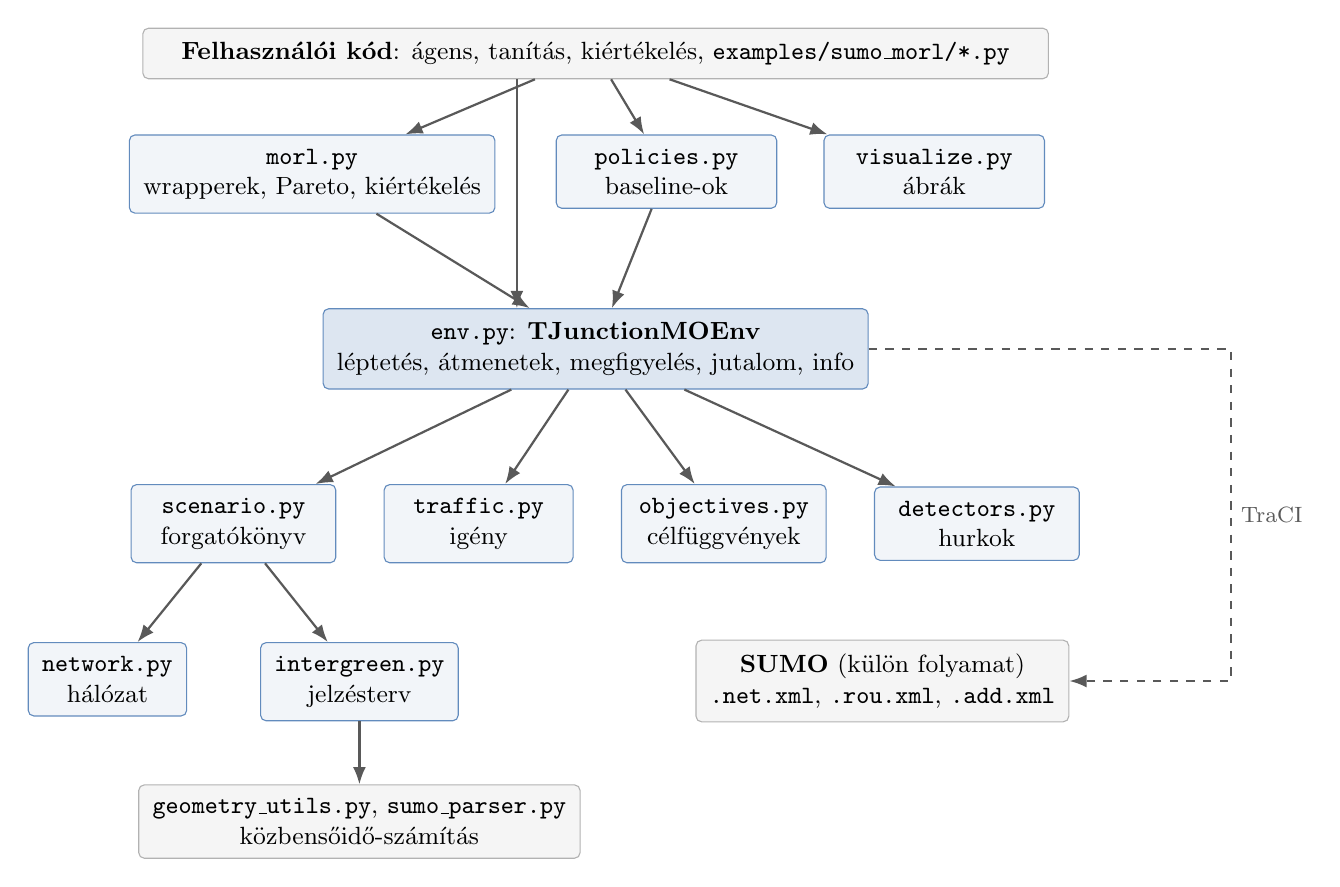
\begin{tikzpicture}[node distance=7mm and 6mm]
  \node[kulso,minimum width=11.5cm] (user) {\textbf{Felhasználói kód}: ágens, tanítás, kiértékelés, \kod{examples/sumo\_morl/*.py}};
  \node[doboz,below=of user,xshift=-3.6cm,minimum width=4.2cm] (morl) {\kod{morl.py}\\wrapperek, Pareto, kiértékelés};
  \node[doboz,below=of user,xshift=0.9cm,minimum width=2.8cm] (pol) {\kod{policies.py}\\baseline-ok};
  \node[doboz,below=of user,xshift=4.3cm,minimum width=2.8cm] (vis) {\kod{visualize.py}\\ábrák};
  \node[doboz,below=12mm of morl,xshift=3.6cm,minimum width=6cm,fill=fokek!15] (env) {\kod{env.py}: \textbf{TJunctionMOEnv}\\léptetés, átmenetek, megfigyelés, jutalom, info};
  \node[doboz,below=12mm of env,xshift=-4.6cm,minimum width=2.6cm] (scen) {\kod{scenario.py}\\forgatókönyv};
  \node[doboz,right=of scen,minimum width=2.4cm] (traf) {\kod{traffic.py}\\igény};
  \node[doboz,right=of traf,minimum width=2.6cm] (obj) {\kod{objectives.py}\\célfüggvények};
  \node[doboz,right=of obj,minimum width=2.6cm] (det) {\kod{detectors.py}\\hurkok};
  \node[doboz,below=10mm of scen,xshift=-1.6cm] (net) {\kod{network.py}\\hálózat};
  \node[doboz,below=10mm of scen,xshift=1.6cm] (ig) {\kod{intergreen.py}\\jelzésterv};
  \node[kulso,below=8mm of ig] (geo) {\kod{geometry\_utils.py}, \kod{sumo\_parser.py}\\közbensőidő-számítás};
  \node[kulso,below=10mm of det,xshift=-1.2cm,minimum width=4.6cm] (sumo) {\textbf{SUMO} (külön folyamat)\\\kod{.net.xml}, \kod{.rou.xml}, \kod{.add.xml}};
  \draw[nyil] (user) -- (morl);
  \draw[nyil] (user) -- (pol);
  \draw[nyil] (user) -- (vis);
  \draw[nyil] (user.south -| -1,0) -- (env.north -| -1,0);
  \draw[nyil] (morl) -- (env);
  \draw[nyil] (pol) -- (env);
  \draw[nyil] (env) -- (scen);
  \draw[nyil] (env) -- (traf);
  \draw[nyil] (env) -- (obj);
  \draw[nyil] (env) -- (det);
  \draw[nyil] (scen) -- (net);
  \draw[nyil] (scen) -- (ig);
  \draw[nyil] (ig) -- (geo);
  \draw[nyil,dashed] (env.east) -- ++(4.6,0) |- node[pos=0.25,right,font=\footnotesize] {TraCI} (sumo.east);
\end{tikzpicture}
\caption{A modulok és függőségeik. A nyíl jelentése: \enquote{használja}.}
\label{fig:retegek}
\end{figure}

%======================================================================
\section{Könyvtárszerkezet}

\begin{lstlisting}[style=bash,basicstyle=\ttfamily\footnotesize]
sumo_morl/                  a könyvtár
    __init__.py             nyilvános API, gym-regisztráció (sumo_morl/TJunction-v0)
    env.py                  TJunctionMOEnv - a Gymnasium környezet
    scenario.py             TJunctionScenario - hálózat + jelzésterv + detektorok
    network.py              a T-csomópont hálózatának generálása netconvert-tel
    intergreen.py           jelzőcsoportok, fázisok, átmenetek a közbenső időkből
    detectors.py            hurokdetektorok: elhelyezés, olvasás, aggregálás
    traffic.py              Demand - forgalmi igény, route fájl írása
    objectives.py           célfüggvények regisztere
    policies.py             összehasonlító vezérlők
    morl.py                 skalarizálás, súlyok, Pareto, hipertérfogat, kiértékelés
    visualize.py            ábrák
    sumo_utils.py           SUMO-binárisok megkeresése
    data/t_junction.net.xml a kész hálózat
    tests/                  pytest tesztek
geometry_utils.py           közbensőidő-számítás: pályák, ütközési pontok, idők
sumo_parser.py              közbensőidő-számítás: .net.xml beolvasása
examples/sumo_morl/         demó és példaprogramok
docs/sumo_morl/             dokumentáció (Markdown, LaTeX, API-referencia)
pyproject.toml              telepítési leíró
\end{lstlisting}

%======================================================================
\section{Modulok és felelősségek}

\begin{center}
\begin{tabularx}{\linewidth}{@{}l>{\raggedright\arraybackslash}X>{\raggedright\arraybackslash}p{4.2cm}@{}}
\toprule
Modul & Felelősség & Fő elemek \\
\midrule
\kod{env.py} & a SUMO indítása és léptetése, az akciók végrehajtása (átmenetekkel), a
  megfigyelés, a jutalom és az \kod{info} előállítása & \kod{TJunctionMOEnv} \\
\kod{scenario.py} & a forgatókönyv összeállítása: hálózat, jelzésterv rögzített fázissorrenddel és
  nevekkel, detektorlista & \kod{TJunctionScenario} \\
\kod{intergreen.py} & a közbensőidő-számítás eredményéből jelzőcsoportok, csoportszintű közbensőidő-mátrix,
  fázisok és átmenetek & \kod{SignalPlan}, \kod{build\_signal\_plan} \\
\kod{detectors.py} & a hurkok helyének kiszámítása, az \kod{.add.xml} írása, másodpercenkénti
  olvasás, lépésenkénti aggregálás & \kod{DetectorReader}, \kod{DetectorSnapshot} \\
\kod{traffic.py} & forgalmi igény megadása, sorsolása, route fájl írása & \kod{Demand} \\
\kod{objectives.py} & a célfüggvények regisztere; a beépített célok & \kod{register\_objective}, \kod{OBJECTIVES} \\
\kod{policies.py} & nem tanuló vezérlők összehasonlításhoz & \kod{FixedTimePolicy}, \kod{ActuatedPolicy}, \dots \\
\kod{morl.py} & MORL-eszközök: wrapperek, súlyok, Pareto, hipertérfogat, epizód futtatása &
  \kod{LinearScalarization}, \kod{evaluate\_policy}, \dots \\
\kod{visualize.py} & ábrák a forgatókönyvről és az epizódokról & \kod{plot\_scenario}, \kod{plot\_signal\_timeline}, \dots \\
\kod{network.py} & a hálózat újragenerálása \kod{netconvert}-tel & \kod{build\_network} \\
\kod{sumo\_utils.py} & a \kod{sumo}, \kod{sumo-gui}, \kod{netconvert} megkeresése & \kod{find\_sumo\_binary} \\
\bottomrule
\end{tabularx}
\end{center}

%======================================================================
\section{Fő osztályok és adatszerkezetek}

\subsection{\kod{TJunctionMOEnv} (\kod{env.py})}

A \kod{gymnasium.Env} leszármazottja.

\begin{center}
\begin{tabularx}{\linewidth}{@{}l>{\raggedright\arraybackslash}X@{}}
\toprule
\kod{action\_space} & \kod{Discrete(n\_phases)} \\
\kod{observation\_space} & \kod{Box(0, 1, (55,))} \\
\kod{reward\_space}, \kod{reward\_dim} & a vektor-jutalom tere és hossza \\
\kod{scenario}, \kod{plan}, \kod{detectors} & a forgatókönyv, a jelzésterv, a detektorlista \\
\kod{objective\_names} & a jutalomvektor komponenseinek nevei \\
\kod{reset(seed, options)} & új forgalom, route fájl írása, SUMO (újra)indítása, opcionális bemelegítés \\
\kod{step(action)} & maradás vagy átmenet + minimális zöld; mérés, jutalom, \kod{info} \\
\kod{observation\_names()} & a megfigyelésvektor elemeinek nevei \\
\kod{close()} & a SUMO leállítása, ideiglenes fájlok törlése \\
\midrule
\kod{\_run\_green(s)} & az aktuális fázis zöldjének futtatása \kod{s} másodpercig \\
\kod{\_run\_transition(p)} & átmenet a \kod{p} fázisba a \kod{SignalPlan.transition} szerint \\
\kod{\_sim\_step()} & egy szimulációs másodperc: \kod{simulationStep}, detektorolvasás, valós mutatók \\
\kod{\_observation(snap)} & a megfigyelésvektor összeállítása és normalizálása \\
\kod{\_gt\_sample()} & valós mutatók gyűjtése (csak \kod{info}-ba) \\
\bottomrule
\end{tabularx}
\end{center}

Minden példány saját ideiglenes munkakönyvtárat (route- és detektorfájl) és egyedi TraCI-címkét
használ, ezért több példány futhat egyszerre.

\subsection{\kod{SignalPlan} (\kod{intergreen.py})}

\begin{center}
\begin{tabularx}{\linewidth}{@{}l>{\raggedright\arraybackslash}X@{}}
\toprule
\kod{links} & a SUMO linkek (\kod{Link}: index, honnan, sáv, hova, irány) \\
\kod{groups} & jelzőcsoportok (\kod{SignalGroup}: név, sáv, linkek) \\
\kod{phases} & fázisonként a zöldet kapó csoportok indexei \\
\kod{intergreen} & csoportszintű közbensőidő-mátrix \kod{[kiürítő, belépő]}, \kod{nan} = nincs konfliktus \\
\kod{link\_intergreen} & a link-szintű mátrix, ahogy a közbensőidő-számítás adta \\
\kod{green\_state(p)} & a \kod{p} fázis SUMO-állapotsztringje (pl. \kod{GrrrGG}) \\
\kod{transition(a, b)} & \kod{[(állapot, időtartam), ...]} az \kod{a}$\to$\kod{b} átmenethez \\
\kod{describe()} & szöveges összefoglaló \\
\bottomrule
\end{tabularx}
\end{center}

\subsection{\kod{DetectorSnapshot} (\kod{detectors.py})}

Egy vezérlési lépés aggregált hurokadatai. A tömbök a detektorlista sorrendjét követik.

\begin{center}
\begin{tabularx}{\linewidth}{@{}l>{\raggedright\arraybackslash}X@{}}
\toprule
\kod{duration} & a lépés hossza [s] \\
\kod{count}, \kod{occupancy}, \kod{speed}, \kod{gap} & áthaladások, átlagos foglaltság, átlagsebesség, időrés \\
\kod{approach\_vehicles} & bemenet--kimenet becslés ágankként a lépés végén \\
\kod{approach\_vehicle\_seconds} & a becslés időintegrálja a lépés alatt \\
\kod{stopline\_occupied\_seconds} & foglalt másodpercek detektoronként \\
\kod{select(kind, lane\_id, approach)} & logikai maszk a szűréshez \\
\bottomrule
\end{tabularx}
\end{center}

\subsection{További osztályok}

\begin{itemize}
  \item \kod{TJunctionScenario}: \kod{net\_file}, \kod{plan}, \kod{detectors}; a fázissorrendet és a
        neveket a \kod{PHASE\_LANES}, \kod{PHASE\_NAMES} konstansok rögzítik, és ellenőrzi, hogy ezek
        pontosan a számolt klikkek.
  \item \kod{Demand}: \kod{flows} (mozgás $\to$ jármű/óra), \kod{profile} (időbeli szorzók);
        \kod{constant}, \kod{random}, \kod{scaled}, \kod{write\_routes}.
  \item \kod{Objective}: név, függvény, skála, leírás; a regiszter az \kod{OBJECTIVES} szótár.
  \item \kod{Policy} és leszármazottai: \kod{\_\_call\_\_(obs, info) -> akció}, \kod{reset()}.
  \item \kod{LinearScalarization}, \kod{WeightConditioned}: \kod{gymnasium} wrapperek.
  \item \kod{EpisodeResult}: \kod{vector\_return}, \kod{ground\_truth}, \kod{history}.
\end{itemize}

%======================================================================
\section{Működés}

\subsection{A jelzésterv előállítása}

A jelzésterv a környezet létrehozásakor, a \kod{TJunctionScenario} konstruktorában készül
(\ref{fig:jelzesterv}.~ábra).

\begin{figure}[h]
\centering
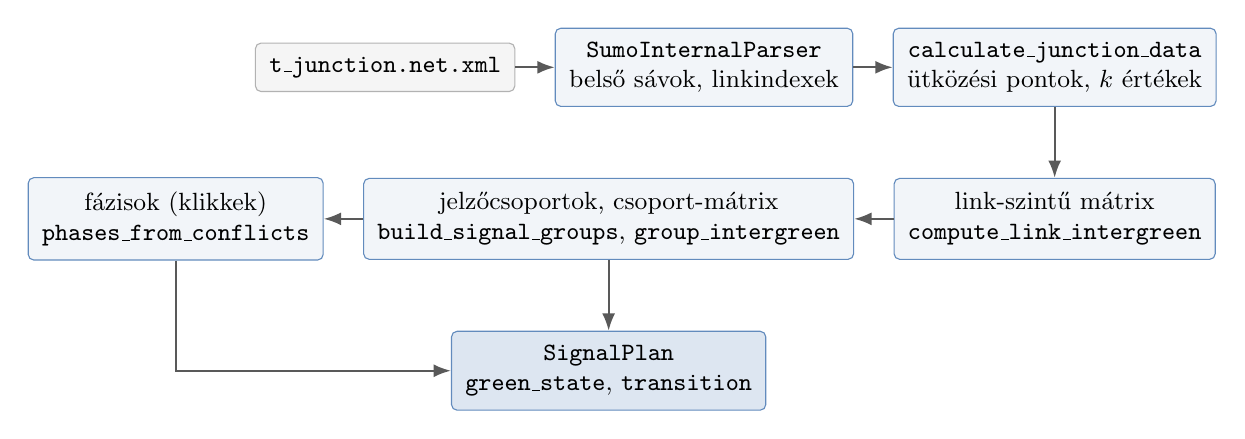
\begin{tikzpicture}[node distance=5mm,font=\small]
  \node[kulso] (n) {\kod{t\_junction.net.xml}};
  \node[doboz,right=of n] (p) {\kod{SumoInternalParser}\\belső sávok, linkindexek};
  \node[doboz,right=of p] (g) {\kod{calculate\_junction\_data}\\ütközési pontok, $k$ értékek};
  \node[doboz,below=9mm of g] (l) {link-szintű mátrix\\\kod{compute\_link\_intergreen}};
  \node[doboz,left=of l] (c) {jelzőcsoportok, csoport-mátrix\\\kod{build\_signal\_groups}, \kod{group\_intergreen}};
  \node[doboz,left=of c] (f) {fázisok (klikkek)\\\kod{phases\_from\_conflicts}};
  \node[doboz,below=9mm of c,fill=fokek!15] (s) {\kod{SignalPlan}\\\kod{green\_state}, \kod{transition}};
  \draw[nyil] (n) -- (p); \draw[nyil] (p) -- (g); \draw[nyil] (g) -- (l);
  \draw[nyil] (l) -- (c); \draw[nyil] (c) -- (f); \draw[nyil] (f) |- (s); \draw[nyil] (c) -- (s);
\end{tikzpicture}
\caption{A jelzésterv előállítása a hálózati fájlból.}
\label{fig:jelzesterv}
\end{figure}

\begin{enumerate}
  \item A \kod{SumoInternalParser} beolvassa a csomópont belső sávjait és linkindexeit.
  \item A \kod{calculate\_junction\_data} (közbensőidő-számítás) megkeresi a pályák ütközési pontjait,
        és mozgáspáronként kiszámolja a közbenső időt.
  \item A \kod{compute\_link\_intergreen} ebből linkindex szerint rendezett mátrixot készít. Ha egy
        párra csak az egyik irányban talált ütközési pontot, a másik irányt is konfliktusnak veszi.
  \item A \kod{build\_signal\_groups} bejövő sávonként egy jelzőcsoportot képez, a
        \kod{group\_intergreen} a csoportok linkjei közötti maximumot veszi.
  \item A \kod{phases\_from\_conflicts} a konfliktusmentes csoportok maximális klikkjeit adja.
  \item A \kod{SignalPlan.transition} két fázis között másodperc pontossággal előállítja az
        átmenetet: a megszűnő csoportok \kod{yellow} ideig sárgát kapnak; az induló $j$ csoport zöldje
        $t_j = \max(\text{red\_yellow},\ \max_i k(i\to j))$ időpontban kezdődik, előtte
        \kod{red\_yellow} ideig piros-sárga; a teljes hossz $\max(\text{yellow}, \max_j t_j)$.
\end{enumerate}

A tesztek (\kod{tests/test\_plan.py}) minden fázispárra ellenőrzik, hogy a közbenső idők teljesülnek,
és hogy zöld után mindig sárga, zöld előtt mindig piros-sárga következik.

\subsection{Egy lépés adatfolyama}

\begin{figure}[h]
\centering
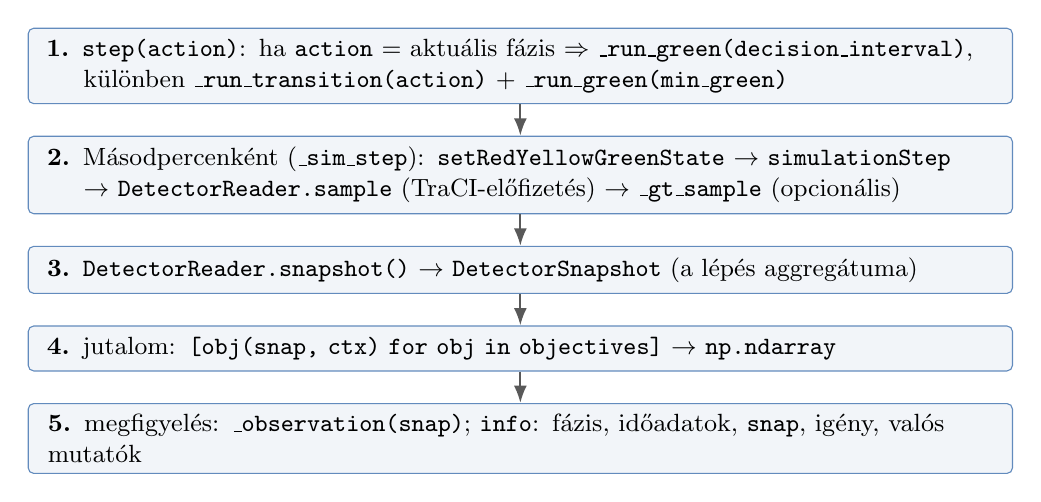
\begin{tikzpicture}[font=\small,
  sor/.style={draw=fokek!70,fill=fokek!6,rounded corners=2pt,minimum width=12.5cm,align=left,inner sep=4pt,text width=12cm}]
  \node[sor] (a) at (0,0) {\textbf{1.} \kod{step(action)}: ha \kod{action} = aktuális fázis $\Rightarrow$ \kod{\_run\_green(decision\_interval)},\\
     \phantom{\textbf{1.} }különben \kod{\_run\_transition(action)} + \kod{\_run\_green(min\_green)}};
  \node[sor,below=4mm of a] (b) {\textbf{2.} Másodpercenként (\kod{\_sim\_step}): \kod{setRedYellowGreenState} $\to$ \kod{simulationStep}\\
     \phantom{\textbf{2.} }$\to$ \kod{DetectorReader.sample} (TraCI-előfizetés) $\to$ \kod{\_gt\_sample} (opcionális)};
  \node[sor,below=4mm of b] (c) {\textbf{3.} \kod{DetectorReader.snapshot()} $\to$ \kod{DetectorSnapshot} (a lépés aggregátuma)};
  \node[sor,below=4mm of c] (d) {\textbf{4.} jutalom: \kod{[obj(snap, ctx) for obj in objectives]} $\to$ \kod{np.ndarray}};
  \node[sor,below=4mm of d] (e) {\textbf{5.} megfigyelés: \kod{\_observation(snap)}; \kod{info}: fázis, időadatok, \kod{snap}, igény, valós mutatók};
  \foreach \x/\y in {a/b,b/c,c/d,d/e} \draw[nyil] (\x) -- (\y);
\end{tikzpicture}
\caption{Egy \kod{step()} hívás lépései.}
\end{figure}

A detektorolvasás másodpercenként történik. A \kod{DetectorReader} a hurkon lévő járművek halmazának
változásából számolja az áthaladásokat (felfutó élek), átlagolja a foglaltságot és a sebességet, és
vezeti a bemenet--kimenet becslést ágankként. A \kod{snapshot()} lezárja a lépést, és új gyűjtést
kezd; a becsült járműszám (\kod{approach\_vehicles}) lépéseken át megmarad.

\subsection{Epizód kezdete}

A \kod{reset()} leállítja az előző SUMO-folyamatot, kisorsolja (vagy átveszi) a forgalmi igényt,
megírja a route fájlt, elindítja a SUMO-t a hálózattal, a route fájllal és a detektorfájllal, majd
feliratkozik a hurkok változóira. Ezután beállítja a 0. fázist, és ha \kod{warmup} $>0$, fix idejű
programmal bemelegíti a csomópontot. A bemelegítés jutalma nem számít bele az epizódba.

\subsection{Determinizmus}

A környezet saját véletlengenerátora (\kod{numpy.random.Generator}) a \kod{reset(seed=\dots)}
hívásra újrainicializálódik. Ebből sorsolja az igényt és a SUMO \kod{--seed} értékét, így azonos
\kod{seed} azonos szimulációt ad (ezt teszt ellenőrzi).

%======================================================================
\section{Kiterjesztési pontok}

\begin{description}[style=nextline,leftmargin=1.5em]
  \item[Új célfüggvény] \kod{@register\_objective(név, scale, doc)} dekorátorral; a függvény
    \kod{(DetectorSnapshot, ctx) -> float}. Ezután a név megadható az \kod{objectives} listában.
  \item[Új megfigyelés] \kod{gymnasium.ObservationWrapper}, amely az \kod{obs}-ból vagy az
    \kod{info["detectors"]}-ből dolgozik.
  \item[Új skalarizálás] \kod{gymnasium.Wrapper}, amely a \kod{step} vektor-jutalmát alakítja át (minta:
    \kod{LinearScalarization}).
  \item[Új vezérlő] a \kod{Policy} osztály leszármazottja \kod{\_\_call\_\_(obs, info)} metódussal.
  \item[Más forgalom] \kod{Demand} objektum vagy \kod{rng -> Demand} függvény a \kod{demand}
    paraméterben.
  \item[Más geometria] \kod{network.build\_network(NetworkSpec(...))}, majd
    \kod{TJunctionScenario(net\_file=...)}. Más csomóponttípushoz új forgatókönyv-osztály kell; a
    \kod{build\_signal\_plan} tetszőleges jelzőlámpás csomópontra működik.
\end{description}

%======================================================================
\section{Tesztek és dokumentáció}

\begin{center}
\begin{tabularx}{\linewidth}{@{}l>{\raggedright\arraybackslash}X@{}}
\toprule
\kod{tests/test\_plan.py} & csoportok és fázisok, konfliktusmentesség, közbenső idők betartása minden
  átmenetben, jelzési sorrend \\
\kod{tests/test\_env.py} & terek, Gymnasium env checker, determinizmus, vezérlők, a detektoros becslés
  pontossága a valós értékhez képest, wrapperek, kiértékelés, Pareto és hipertérfogat, jelzésnapló \\
\bottomrule
\end{tabularx}
\end{center}

Futtatás: \kod{python -m pytest} (kb.\ fél perc).

A dokumentáció forrásai: \kod{docs/sumo\_morl/latex/kezikonyv.tex}, \kod{programfelepites.tex};
az API-referencia a docstringekből készül a \kod{pdoc} eszközzel. Mindhárom újragenerálható:

\begin{lstlisting}[style=bash]
pip install pdoc
python docs/sumo_morl/latex/build_docs.py      # PDF-ek + API-referencia (HTML)
\end{lstlisting}

%======================================================================
\newpage
\appendix
\section{A teljes forráskód}
\lstset{style=lista}
% Automatikusan generálva (build_docs.py)
\subsection{Csomag belépési pont}
\kod{sumo\_morl/\_\_init\_\_.py}
\lstinputlisting[language=Python]{\rootdir/sumo_morl/__init__.py}

\subsection{A környezet}
\kod{sumo\_morl/env.py}
\lstinputlisting[language=Python]{\rootdir/sumo_morl/env.py}

\subsection{Forgatókönyv}
\kod{sumo\_morl/scenario.py}
\lstinputlisting[language=Python]{\rootdir/sumo_morl/scenario.py}

\subsection{Jelzésterv a közbenső időkből}
\kod{sumo\_morl/intergreen.py}
\lstinputlisting[language=Python]{\rootdir/sumo_morl/intergreen.py}

\subsection{Hurokdetektorok}
\kod{sumo\_morl/detectors.py}
\lstinputlisting[language=Python]{\rootdir/sumo_morl/detectors.py}

\subsection{Célfüggvények}
\kod{sumo\_morl/objectives.py}
\lstinputlisting[language=Python]{\rootdir/sumo_morl/objectives.py}

\subsection{Forgalmi igény}
\kod{sumo\_morl/traffic.py}
\lstinputlisting[language=Python]{\rootdir/sumo_morl/traffic.py}

\subsection{Összehasonlító vezérlők}
\kod{sumo\_morl/policies.py}
\lstinputlisting[language=Python]{\rootdir/sumo_morl/policies.py}

\subsection{MORL segédfüggvények}
\kod{sumo\_morl/morl.py}
\lstinputlisting[language=Python]{\rootdir/sumo_morl/morl.py}

\subsection{Ábrák}
\kod{sumo\_morl/visualize.py}
\lstinputlisting[language=Python]{\rootdir/sumo_morl/visualize.py}

\subsection{Hálózat generálása}
\kod{sumo\_morl/network.py}
\lstinputlisting[language=Python]{\rootdir/sumo_morl/network.py}

\subsection{SUMO segédfüggvények}
\kod{sumo\_morl/sumo\_utils.py}
\lstinputlisting[language=Python]{\rootdir/sumo_morl/sumo_utils.py}

\subsection{Közbensőidő-számítás: geometria}
\kod{geometry\_utils.py}
\lstinputlisting[language=Python]{\rootdir/geometry_utils.py}

\subsection{Közbensőidő-számítás: hálózat beolvasása}
\kod{sumo\_parser.py}
\lstinputlisting[language=Python]{\rootdir/sumo_parser.py}

\subsection{Demó: fix idejű program}
\kod{examples/sumo\_morl/00\_demo\_fix\_ido.py}
\lstinputlisting[language=Python]{\rootdir/examples/sumo_morl/00_demo_fix_ido.py}

\subsection{Példa: ismerkedés}
\kod{examples/sumo\_morl/01\_ismerkedes.py}
\lstinputlisting[language=Python]{\rootdir/examples/sumo_morl/01_ismerkedes.py}

\subsection{Példa: összehasonlító vezérlők}
\kod{examples/sumo\_morl/02\_baseline\_osszehasonlitas.py}
\lstinputlisting[language=Python]{\rootdir/examples/sumo_morl/02_baseline_osszehasonlitas.py}

\subsection{Példa: súlyozott tanítás (SB3)}
\kod{examples/sumo\_morl/03\_sb3\_sulyozott\_tanitas.py}
\lstinputlisting[language=Python]{\rootdir/examples/sumo_morl/03_sb3_sulyozott_tanitas.py}

\subsection{Példa: saját célfüggvény}
\kod{examples/sumo\_morl/04\_sajat\_celfuggveny.py}
\lstinputlisting[language=Python]{\rootdir/examples/sumo_morl/04_sajat_celfuggveny.py}

\subsection{Tesztek: jelzésterv}
\kod{sumo\_morl/tests/test\_plan.py}
\lstinputlisting[language=Python]{\rootdir/sumo_morl/tests/test_plan.py}

\subsection{Tesztek: környezet}
\kod{sumo\_morl/tests/test\_env.py}
\lstinputlisting[language=Python]{\rootdir/sumo_morl/tests/test_env.py}

\subsection{Telepítési leíró}
\kod{pyproject.toml}
\lstinputlisting[language={}]{\rootdir/pyproject.toml}



\end{document}
